\chapter{Diamond-Square Algorithmus}\label{diamondsquare}
Die Vorteile des Diamond-Square Algorithmus liegen insbesondere in seinen, trotz seiner einfachen Implementierung, optisch plausiblen Ergebnissen. 
Der Algorithmus unterteilt sich pro Rekursionschritt in 2 Phasen\footnote{Auch \emph{Steps} genannt}: der Diamond und der Square Step. Das zu berechnende Höhenfeld muss dabei in der Auflösung eine Breite bzw. Höhe von $2n+1$ wobei $ n\in\mathbb{N}$ aufweisen.

\subsection{Der Algorithmus}
Zur Initialisierung werden den vier Eckpunkte des zu berechnenden Höhenfeldes jeweils zufällige Höhenwerte zugewiesen. Außerdem wird eine von der Rekursionstiefe abhängige Offset-Funktion $O(k)=(rnd()*2-1)/2^k$ definiert, wobei rnd() einen Zufallswert zwischen 0-1(inklusive) zurückgibt und $k$ der Rekursionschritt ist.

Im Diamond Step wird nun der Mittelpunkt des Höhenfeld gesucht und mittels einer beliebigen Interpolation\footnote{In der Beispielimplementierung wurde eine billineare Interpolation gewählt} zwischen den 4 Höhenwerten der Eckpunkte ein Wert ermittelt, welcher dann mit dem Ergebnis der Offset-Funktion addiert wird.
\begin{figure}
	\centering
	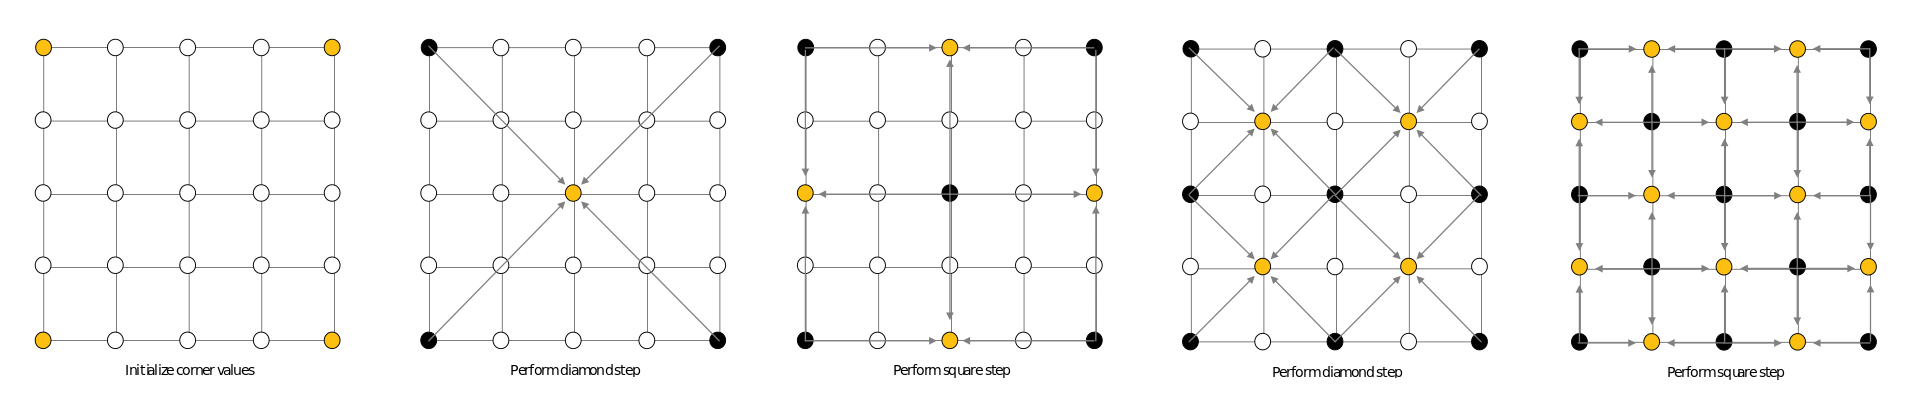
\includegraphics[width=\textwidth]{images/Diamond_Square.png}
	\caption{Diamond Square Algorithmus bei einem quadratischen Höhenfeld mit der Auflösung 5x5. Bildquelle: http://tinyurl.com/h29sv48}\label{img.dmsquare}
\end{figure}
Bei dem Square Step werden nun die jeweiligen mittleren Randpunkte zwischen den bereits initialisierten Eckpunkten durch eine einfache Interpolation zwischen den 2 nächstliegendsten Eckpunkten berechnet.
Wie in \autoref{img.dmsquare} zu sehen ergeben sich daraus 4 weitere Vierecke mit berechneten Eckpunkten, auf die der Algorithmus erneut angewandt wird. Dies wird solange wiederholt, bis alle Vertices berechnet sind.
%TODO Ab hieor weiterchecken
\subsection{Flexibilität}
Das resultierende Höhenfeld lässt sich einfach durch eine Veränderung der Offset-Funktion relativ flexibel anpassen. So besteht zum Beispiel die Möglichkeit, die Offset-Funktion von dem interpolierten Höhenwert des aktuellen Punktes abhängig so machen und dadurch ein heterogenes Landschaftsbild zu erzeugen.

\subsection{Bewertung im Rahmen der Fragestellung}
Zur Speicherung des resultierenden Höhenfeldes reicht es aus den Seed\footnote{Eingangswert für einen Pseudozufallsgenerator. https://www.wikiwand.com/en/Random\_seed} des Pseudozufallsgenerators sowie die vier initialen Werte zu speichern. Eine Landschaft wie sie etwa Minecraft bietet wäre mit diesem Algorithmus aus 2 Gründen allerdings nicht möglich. Wie bereits besprochen verwendet Minecraft Voxel, welche mit dem Diamond Square Algorithmus allerdings nicht berechnet werden können. Außerdem würde die Generierung der Spielwelt besonders für Spieler mit Leistungsschwachen Computern sehr lange dauern. Um das zu vermeiden könnte man die Landschaft in rechteckige Patches\footnote{Kleine Abschnitte der Landschaft einzeln berechnen und aneinanderfügen} aufteilen, die erst berechnet werden wenn der Spieler auf sie tritt. Da der Pseudozufallsgenerator jedoch seine Werte immer in der gleichen Reihenfolge ausgibt wäre die Anordnung der Patches zueinander abhängig von der Reihenfolge in der sie geladen werden\label{Patches}.

\lstinputlisting[language=csh, title=Diamond-Square Implementierung C\#]{data/diamondSquare.cs}